\customsection{User app}

Teniendo en miras de la escalabilidad deseada para este sistema se escogió el framework de desarrollo de aplicaciones móviles llamado React Native. Este es un framework de JavaScript desarrollado y mantenido por Facebook Inc con ventajas significativas desde la perspectiva de diseño: permite desarrollar aplicaciones nativas para Android y iOS a través de un sistema de traducción de componentes desde JavaScript al lenguaje nativo de la maquina (Java para Android y Swift para IOS), por ende, las aplicaciones desarrolladas en este framework tienen un desempeño muy similar a las implementadas directamente en los lenguajes nativos correspondientes.
\vspace{0.5cm}\\
En adición, una ventaja estratégica que tiene el desarrollar aplicaciones a través de este framework es que ambos desarrollos (para IOS y Android) quedan con las mismas interfaces gráficas, lo que le da al cliente la misma experiencia de usuario sin importar en que plataforma se encuentre.
\vspace{0.5cm}\\
Aunque desarrollar aplicaciones para Android y IOS con el mismo lenguaje de programación suena extremadamente ventajoso, hay limitaciones técnicas que serán mencionadas más adelante en este capítulo.

\subsection{Especificaciones técnicas}

Para poder realizar el aplicativo se utilizaron diferentes librerías de JavaScript creadas específicamente para el framework de React-Native. Las librerías utilizadas en el aplicativo fueron:

\begin{itemize}
	\item \textbf{React-native-google-signin:} Esta librería fue utilizada para obtener las llaves privadas y la información de usuario utilizando el servicio de autenticación de Google.
	\item \textbf{React-native-progress:} Con esta librería se lograron desarrollar los indicadores de progreso circulares para mostrar el índice de consumo eléctrico de agua y el coeficiente de sostenibilidad.
	\item \textbf{Jsrsasign:} Usando esta librería fue posible encriptar los JWT de autenticación a partir del protocolo de RSA de 256 bits. Esta librería fue de vital importancia puesto que poseía toda la compatibilidad necesaria para ser ejecutada con JavaScript puro, sin el uso de paquetes adicionales escritos en Java o Swift.
	\item \textbf{React-native-svg:} Esta librería fue utilizada para apoyar el desarrollo de componentes visuales adicionados a las gráficas.
	\item \textbf{React-native-svg-charts:} Usando esta librería fue posible integrar gráficas en el aplicativo móvil.
	\item \textbf{React-native-swiper:} Con esta librería se implementó la interfaz tipo deslizante (``swipe'') en las ventanas de introducción de la aplicación.
	\item \textbf{React-native-vector-icons:} Con esta librería fue posible utilizar los iconos nativos de Android y IOS como el botón de menú, de home, entre otros.
	\item \textbf{Toggle-switch-react-native:} Con esta librería se implementaron botones conmutadores (on off), utilizados en la escena de control.
	\item \textbf{React-navigation:} Esta librería fue utilizada para establecer el control de la navegación y el menú dentro de la aplicación como se puede ver en la figura \ref{fig_17}.
	\item \textbf{React-redux:} Usando esta librería fue posible comunicar de manera efectiva todos los objetos y componentes del sistema.
	\item \textbf{Fetch:} Con esta librería se estableció la comunicación basada en solicitudes Https con el backend.
\end{itemize}
\begin{figure}[htbp]
	\centerline{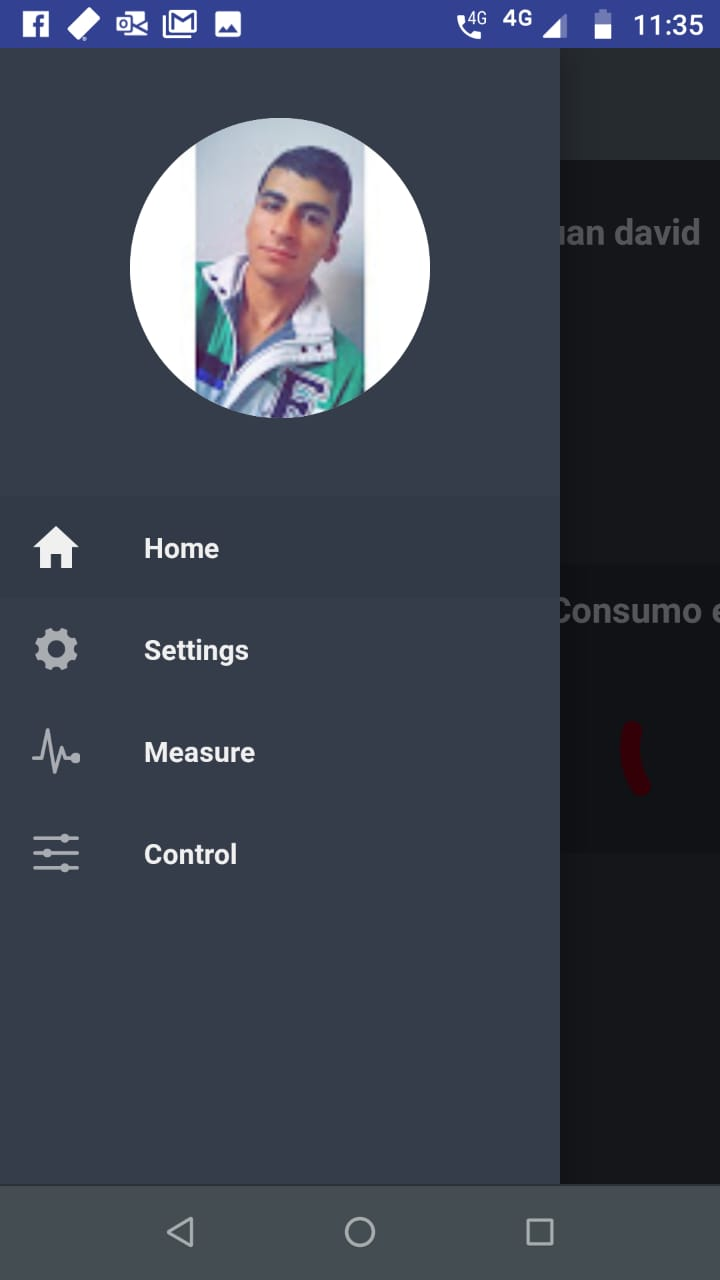
\includegraphics[width=6cm]{./figuras/mobile_menu.jpeg}}
	\caption{El menú desplegable con las aplicaciones actualmente desplegadas. Fuente: propia}
	\label{fig_17}
\end{figure}
Teniendo en cuenta que React\_native traduce todos sus componentes al lenguaje nativo del celular, es necesario entender que no todas las librerías de JavaScript se pueden usar para el framework, únicamente aquellas que tienen incluido el enlace de bajo nivel con ambos sistemas operativos. Por ende, las librerías con mayor compatibilidad son las que están desarrolladas exclusivamente con JavaScript puro. 
\vspace{0.5cm}\\
Con la anterior consideración en mente, en el proceso de desarrollo se presentó un problema por asumir incorrectamente que un ``snipet'' (Archivo o script que cumple una función en específico) era capaz de funcionar en el entorno de programación de React-Native. Este pequeño ``snipet'' fue desarrollado pensando en integrar las funcionalidades del protocolo de comunicación Mqtts a la aplicación; pero usaba librerías que estaban basadas en paquetes de bajo nivel equivocados, es decir, para computadores de uso comercial como linux o windows. Por ende, las funcionalidades de tiempo real fueron implementadas utilizando únicamente el protocolo de comunicación Https.
\vspace{0.5cm}\\
Para finalizar, de las librerías utilizadas, se puede observar que la mayoría son para mejorar la interfaz gráfica, mejorar la experiencia de usuario u obtener la misma vista entre sistemas operativos Android y Ios.

\subsection{Requerimientos Funcionales}

Debido a que durante el proceso de planeación del proyecto también se utilizó la herramienta de RUP para definir las especificaciones de esta aplicación, y estos requerimientos guiaron el proceso de desarrollo, se explicará cómo se implementaron las especificaciones establecidas:

\begin{enumerate}
	\item \textsl{``El usuario debe poder acceder a la información medida en tiempo real:''} Para solucionar este requerimiento, en una primera etapa de desarrollo, se optó por utilizar una librería llamada ``react-native-mqtt''. Esta librería funcionaria como puente entre las librerías: ``Paho Mqtt Client' de Android y ``Mqtt Framework'' de IOS, pero debido al estado tan pionero de las tecnologías de desarrollo de React Native y el protocolo de comunicación Mqtt, la librería no era estable y muchas otras similares tampoco. 
	\vspace{0.5cm}\\
	Teniendo en cuenta lo anterior se implementó la comunicación en ambos sentidos a través de las solicitudes Https, por ende, para obtener los datos en tiempo real en la aplicación le realiza solicitudes al backend de tal forma que reciba los últimos datos guardados en el sistema de almacenamiento MySql.
	\vspace{0.5cm}\\
	Finalmente, para mostrar la información medida en tiempo real se implementó la escena de medición ``measure'' tal como se ve en la figura \ref{fig_15}, donde deslizándose hacia abajo se puede tener acceso a las gráficas con contenido de otros sensores.
	\begin{figure}[htbp]
		\centerline{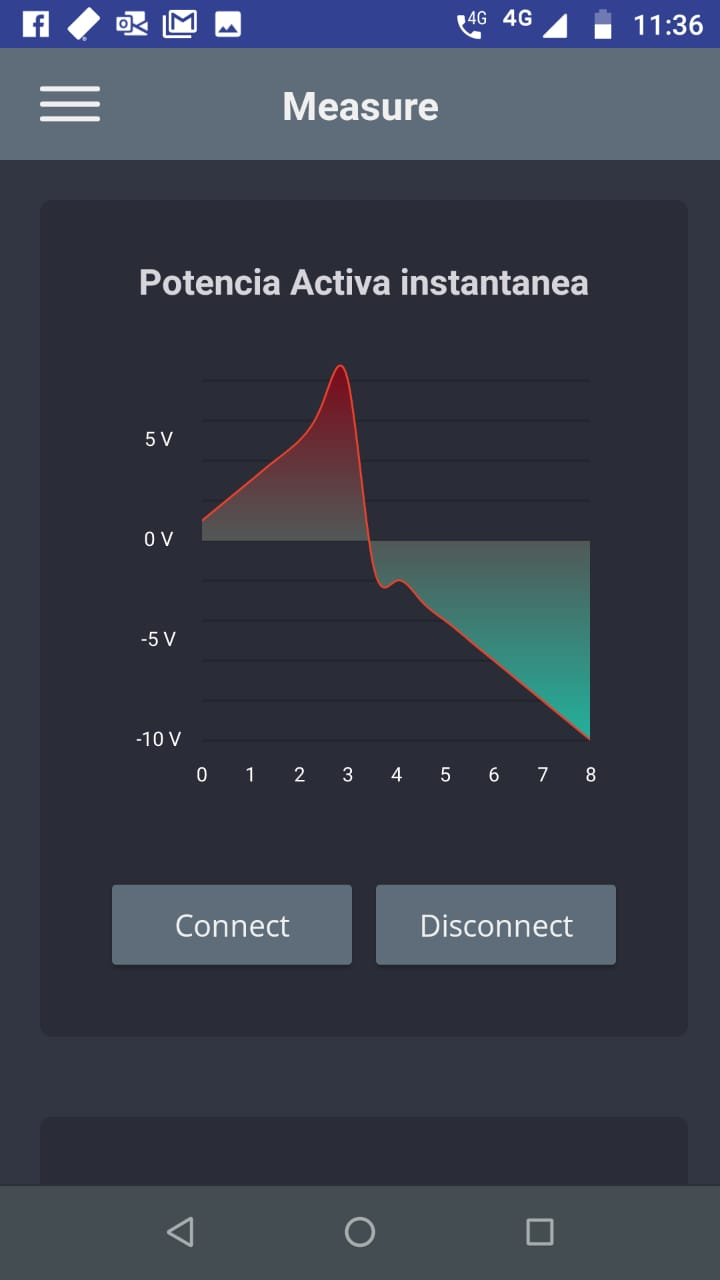
\includegraphics[width=6cm]{./figuras/mobile_measure.jpeg}}
		\caption{Escena para la medición en tiempo real de las variables. Fuente: propia}
		\label{fig_15}
	\end{figure}
	\item  \textit{``El usuario debe ser capaz de cambiar los parámetros de configuraciones establecidos por defecto para la vivienda del solar Decathlon:''} Por defecto los parámetros de la vivienda del Solar Decathlon involucran unos horarios de uso de las cargas eléctricas, por ende, cuando el usuario realiza un cambio en la aplicación celular el sistema en sitio desactiva su configuración predeterminado. 
	\vspace{0.5cm}\\
	Finalmente, se implementó una escena de configuración. Esta escena, no se añadió ninguna entrada de usuario y se dejó para ilustrar la posibilidad de incluirlo en el futuro. La escena se puede observar en la figura \ref{fig_18}.
	
	\begin{figure}[htbp]
		\centerline{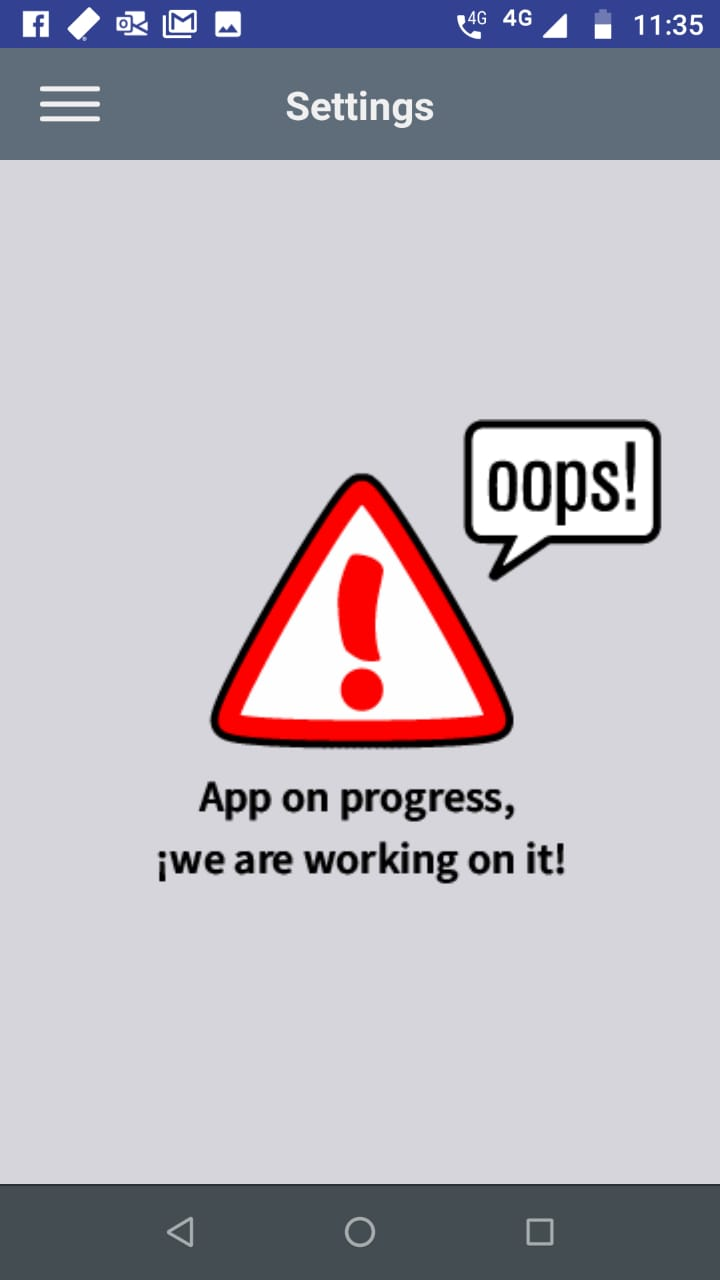
\includegraphics[width=5cm]{./figuras/mobile_settings.jpeg}}
		\caption{Escena de configuraciones, actualmente no disponible. Fuente: propia}
		\label{fig_18}
	\end{figure}
	
	\item \textit{``El usuario debe poder acceder al histórico del mes y la relación de sus gastos con ellos:''} Para implementar este requerimiento se utilizaron barras circulares de progreso que indican la cantidad de energia o agua que ha consumido el usuario en el día, comparándola con un valor promedio. La escena desarrollada para solucionar este requerimiento se puede ver en la figura \ref{fig_13} donde el usuario puede panear horizontalmente el centro de la pantalla para revelar los otros indicadores.
	\begin{figure}[htbp]
		\centerline{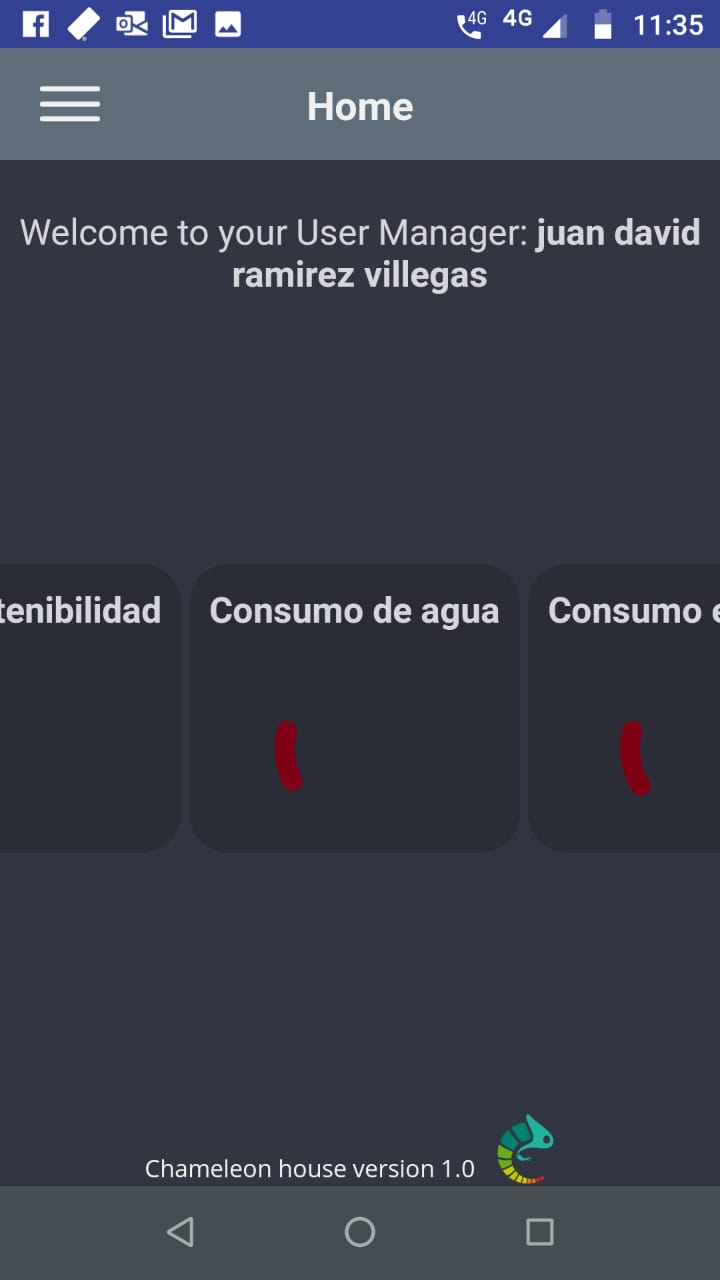
\includegraphics[width=5cm]{./figuras/mobile_home.jpeg}}
		\caption{Escena para la visualización del consumo histórico. Fuente: propia}
		\label{fig_14}
	\end{figure}
	\item  \textit{``La aplicación notificara al usuario cuando la factura este vencida:''} para este requerimiento se implementó una función adicional en el aplicativo en sitio, por ende, para esta versión de la aplicación no se desarrolló ningún componente relacionado con esta necesidad.
	
	\item \textit{``El usuario debe ser capaz de poder ver su impacto ambiental basado en datos cualitativos y cuantitativos:''} Teniendo en cuenta la figura \ref{fig_14} uno de los indicadores corresponde a un indicador de sostenibilidad que está basado en la huella de carbono del consumo de agua y el consumo eléctrico, pero el componente cualitativo no fue implementado para esta versión de la aplicación.
	
	\item \textit{``El sistema debe ser capaz de notificar las perdidas eléctricas y por consiguiente económicas de un mal uso de los horarios establecidos por defecto:''} Para implementar este requerimiento se desarrolló en el aplicativo en sitio la función de notificación automática.
	
\end{enumerate}


\subsection{Funciones adicionales}

En adición a los requerimientos funcionales se añadieron características a la conceptualización de diseño original, lo anterior, para mejorar el funcionamiento de la plataforma y la experiencia de usuario. Estas funciones se pueden ver a continuación:

\begin{enumerate}
	\item \textbf{Pantalla de control:} Teniendo en cuenta un diseño con el mayor control y administración de los actuadores y sensores conectados al sistema, para esta versión de la aplicación, se implementó una interfaz de control que se puede observar en la figura \ref{fig_16}, donde el usuario tiene la posibilidad de modificar la configuración horaria programada por defecto para el Solar Decathlon. Una vez el usuario altera el estado de los circuitos de la vivienda a través de la ventana, El sistema de agenda local se desactiva por 24 horas para darle la prioridad a lo que defina el usuario.
	
	\begin{figure}[htbp]
		\centerline{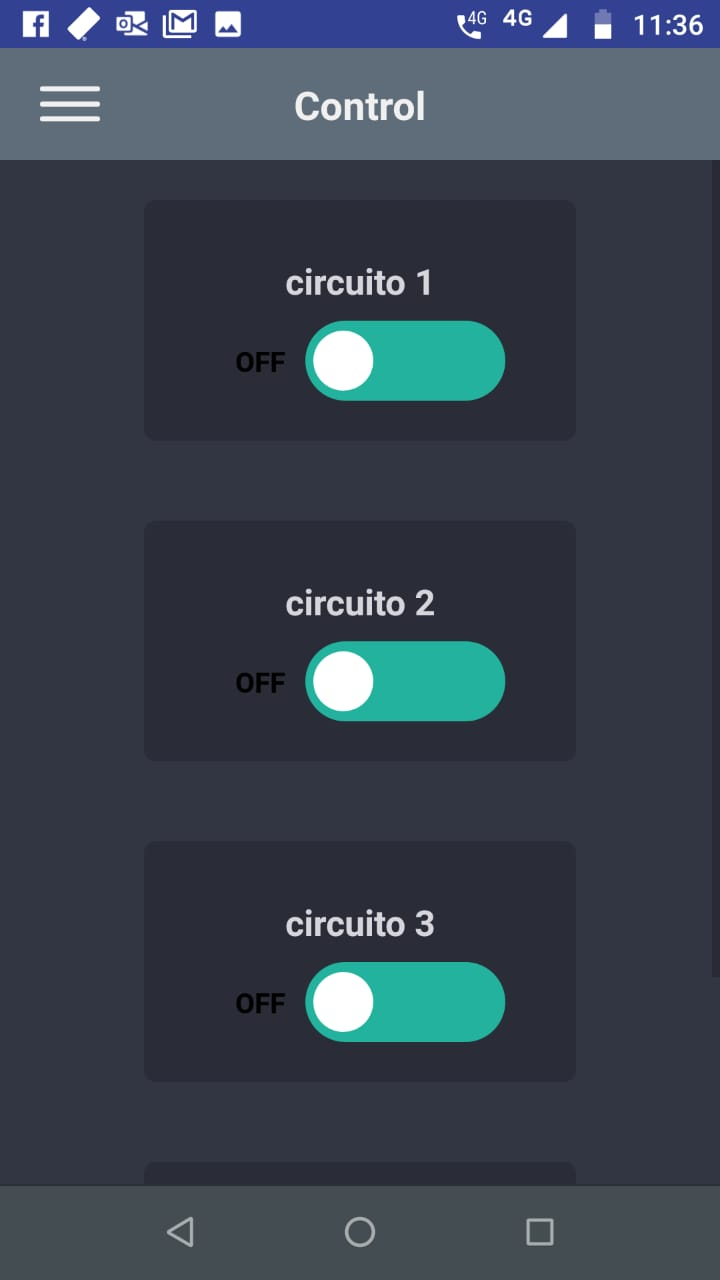
\includegraphics[width=5cm]{./figuras/mobile_control.jpeg}}
		\caption{Escena para el control de los circuitos de la vivienda. Fuente: propia}
		\label{fig_16}
	\end{figure}
	
	\item \textbf{Ventana de introducción:} Esta función es más un componente decorativo, la escena le da la bienvenida al usuario, mejora la experiencia de usuario y le da status a la interfaz. Figura \ref{fig_12}.
	
	\begin{figure}[htbp]
		\centerline{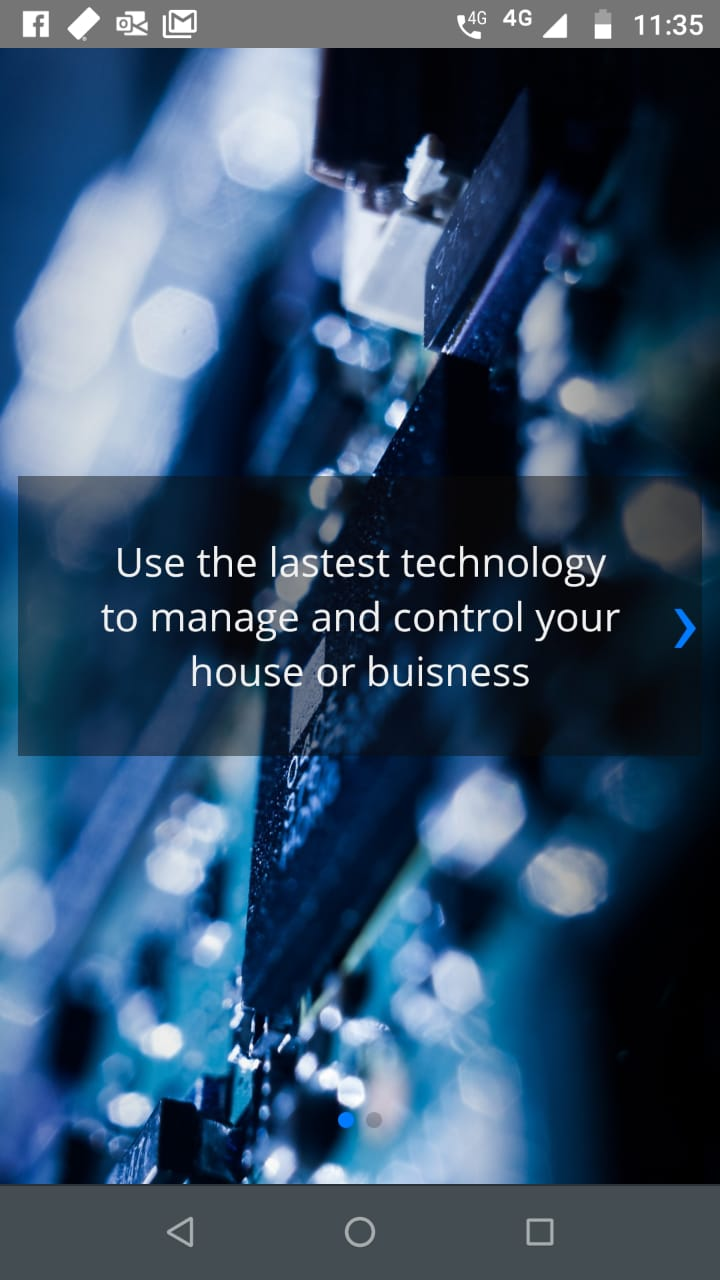
\includegraphics[width=5cm]{./figuras/mobile_intro1.jpeg}}
		\caption{Escena de bienvenida 1. Fuente: propia}
		\label{fig_12}
	\end{figure}
	
	\item \textbf{Servicio de autenticación:} Finalmente, se implementó un servicio de autenticación utilizando la api de Google, utilizando su api de autenticación se desarrolló la interfaz para obtener la información del usuario como: correo, numero de teléfono, nombre completo y una llave encriptada con la que la app puede re autenticar el usuario en caso de ser necesario tal como se ve en la figura \ref{fig_13}.
	
	\begin{figure}[htbp]
		\centerline{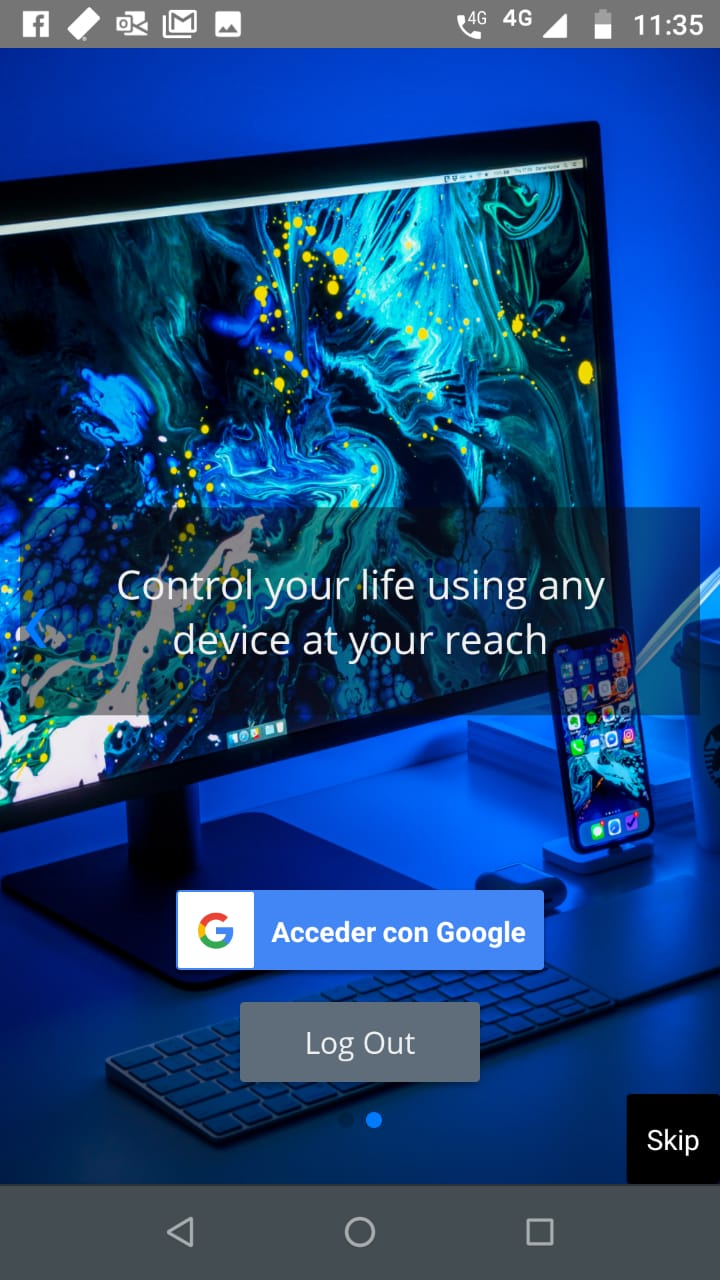
\includegraphics[width=5cm]{./figuras/mobile_intro2.jpeg}}
		\caption{Escena de inicio de sesión. Fuente: propia}
		\label{fig_13}
	\end{figure}	
\end{enumerate}

\subsection{Pruebas de concepto}
Para finalizar, debido a que el sistema desarrollado está constituido enteramente por software se decidió adicionar un componente de hardware para probar conceptualmente la capacidad de añadir cualquier sistema de medición o actuación.
\vspace{0.5cm}\\
Como dispositivo de medición se utilizó un medidor bifásico de la empresa Inelca con una interfaz de comunicación Rs485 \ref{32}. Utilizando esta interfaz y un conversor USB a Rs485 se logró comunicar la Raspberry con el medidor de Inelca.
\vspace{0.5cm}\\
\begin{figure}[htbp]
	\centerline{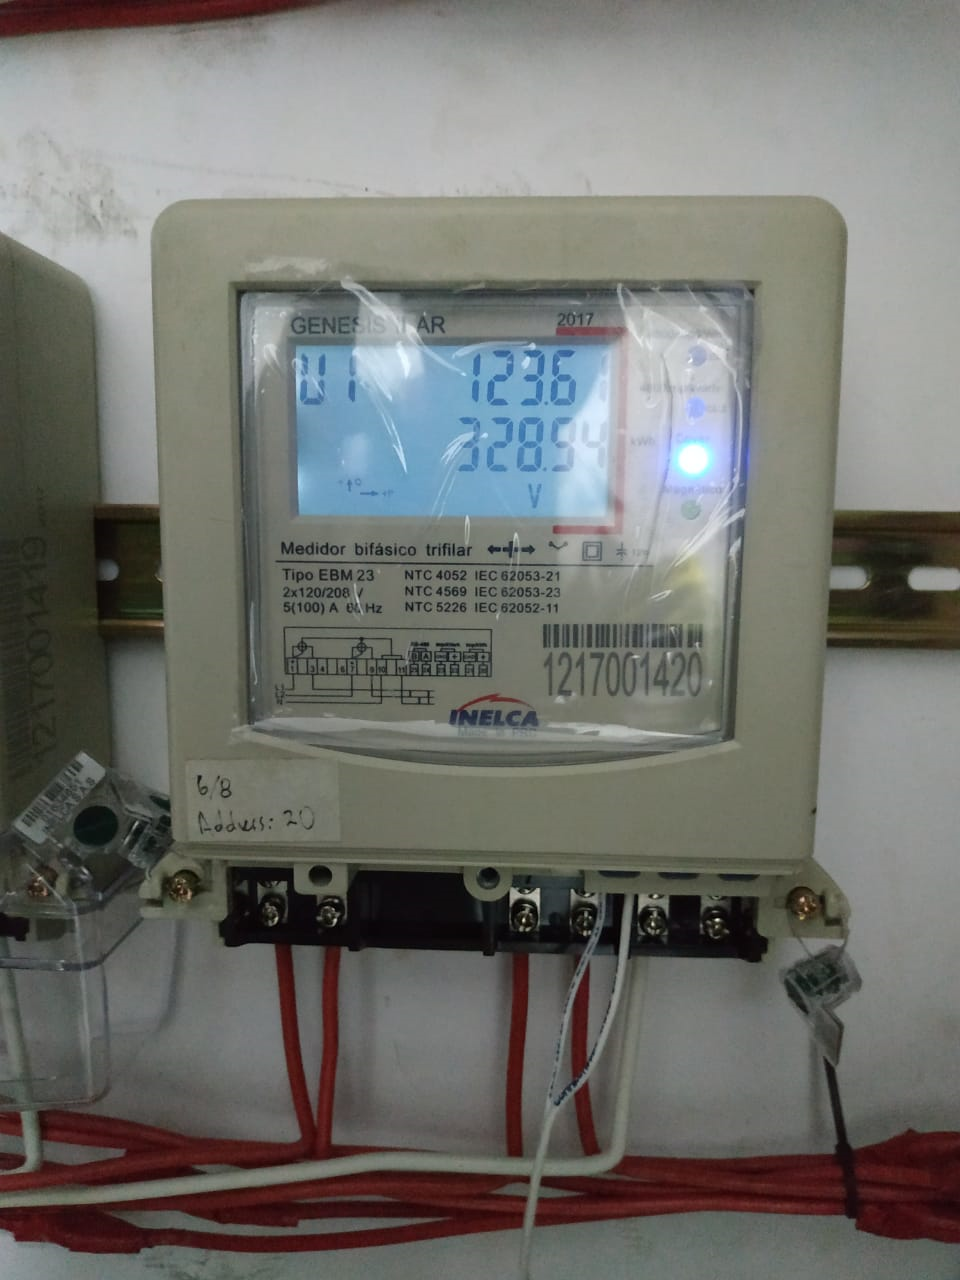
\includegraphics[width=5cm]{./figuras/concepto_1.png}}
	\caption{Dispositivo Inelca utilizado para la prueba de concepto. Fuente: propia}
	\label{fig_32}
\end{figure}

Para finalizar, se puso a prueba el sistema añadiendo la función de adquisición necesaria para obtener el valor del voltaje Rms del medidor a partir de una trama serial tipo modbus, tal como se observa en la figura \ref{fig_33}.

\begin{figure}[htbp]
	\centerline{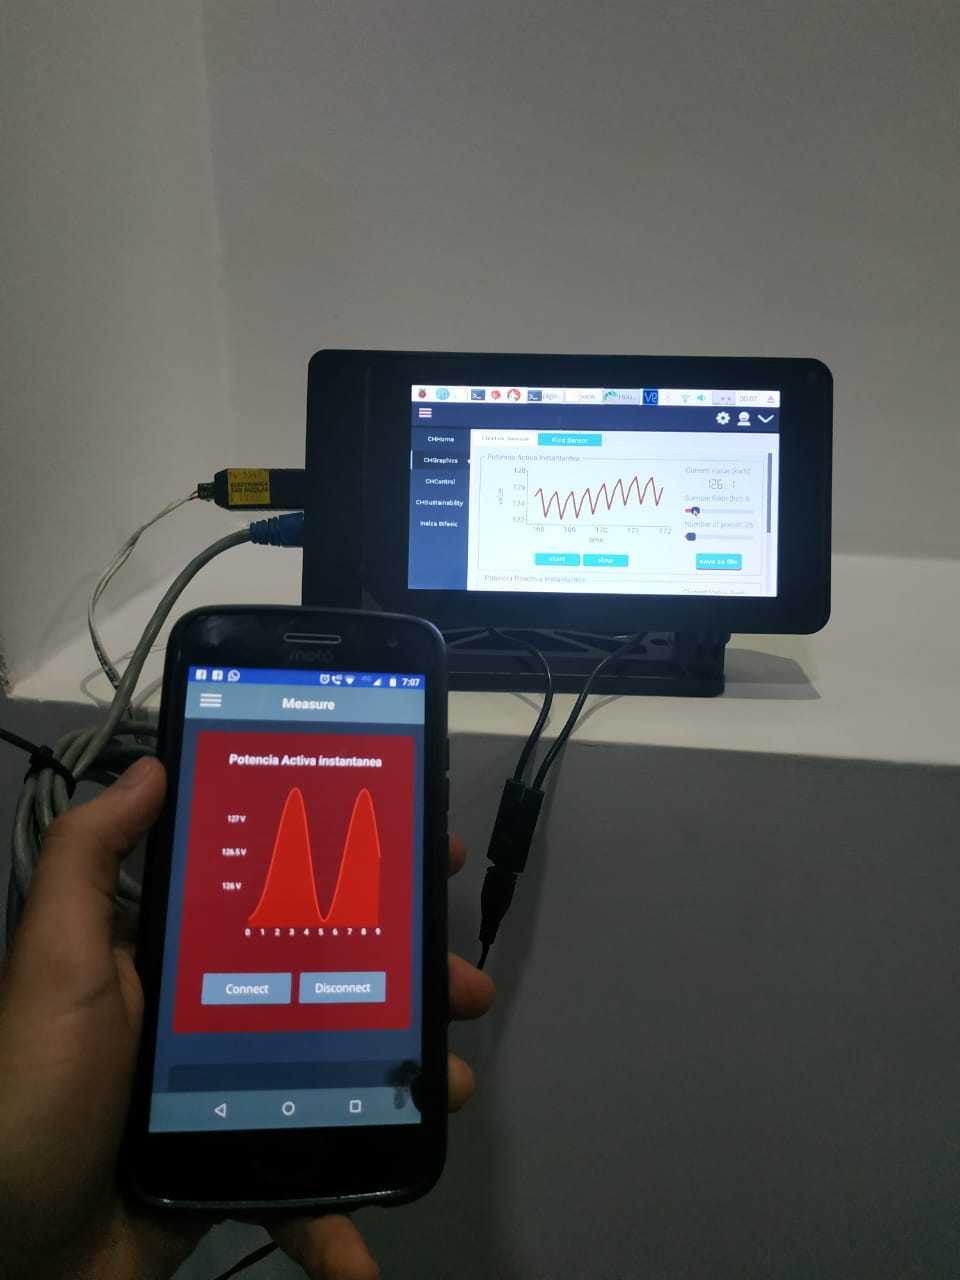
\includegraphics[width=5cm]{./figuras/concepto_2.png}}
	\caption{Prueba de concepto usando todos los sistemas. Fuente: propia}
	\label{fig_33}
\end{figure}
